\section{Taxonomy and Literature Synthesis}\label{sec:taxonomy}

This section answers \texttt{RQ1} by organizing the 47 retained works into six functional classes (\texttt{L1.A--L1.F}) and mapping empirical intersections across phase awareness and carbon/energy signals.

\subsection{Dual-Axis Taxonomy (\texorpdfstring{\texttt{L1.A--L1.F}}{L1.A-L1.F})}\label{subsec:taxonomy_classes}

\subsubsection{L1.A Prior Surveys and Taxonomies (\texorpdfstring{$n=9$}{n=9})}
Recent surveys cover cloud carbon scheduling or LLM efficiency separately without documenting the combined design space (Table~\ref{tab:surveys}). Hewage et al.~\cite{hewage2026carbon} synthesize operational and embodied carbon control for latency-sensitive clouds without mentioning LLMs, prefill/decode, or KV caching. Yang et al.~\cite{yang2025container} review container orchestration across serverless and GPU workloads while omitting disaggregation and embodied carbon. Alam et al.~\cite{alam2026computing} report that 70\% (44/63) of surveyed carbon-aware cloud studies rely solely on simulation and only 6.3\% (4/63) track live grid intensity. Among serverless reviews, Agarwal et al.~\cite{agarwal2026serverless} find sustainability metrics in only 4 of 40 dynamic resource schemes, and Besozzi et al.~\cite{besozzi2025serverless} report 29.5\% GPU support across 122 studies alongside only two carbon mentions.

Conversely, LLM serving surveys by Miao et al.~\cite{miao2025serving}, Jiang et al.~\cite{jiang2026kvcache}, and Pan et al.~\cite{pan2025inference} examine KV transfer and disaggregation without operational or embodied carbon accounting, whereas Bai et al.~\cite{bai2026efficiency} cover operational $\text{PUE}\cdot\text{kWh}\cdot\text{CI}$ metrics without phase disaggregation or embodied manufacturing budgets.

\begin{table*}[t]
\centering
\caption{Audit of Prior Surveys and Taxonomies (\texttt{L1.A}, $n=9$) Across Carbon, Embodied, and LLM Disaggregation Axes}
\label{tab:surveys}
\scriptsize
\setlength{\tabcolsep}{4pt}
\begin{tabular}{@{}llllccccl@{}}
\toprule
\textbf{Work} & \textbf{Year} & \textbf{Venue / Status} & \textbf{Primary Scope} & \textbf{Grid CI} & \textbf{Emb.} & \textbf{LLM} & \textbf{P/D \& KV} & \textbf{Verified Gap Summary} \\
\midrule
Hewage et al.~\cite{hewage2026carbon} & 2026 & arXiv Preprint (28 pp.) & Latency-sensitive cloud & \checkmark & \checkmark & $\times$ & $\times$ & 0 LLM/P/D/KV hits; cites $>60\%$ CO$_2$ cut \\
Yang et al.~\cite{yang2025container} & 2025 & arXiv Preprint (35 pp.) & Container orchestration & \checkmark & $\times$ & Min. & $\times$ & Covers SCI, serverless, GPU; 0 P/D/KV/embodied \\
Alam et al.~\cite{alam2026computing} & 2026 & \textit{Computing} (25 pp.) & Cloud carbon RL/heuristic & 6.3\% & $\times$ & $\times$ & $\times$ & 70\% (44/63) sim-only; 0 GPU/LLM/embodied \\
Agarwal et al.~\cite{agarwal2026serverless} & 2026 & \textit{ACM CSUR} (36 pp.) & Serverless adaptation & 4/40 & $\times$ & Min. & $\times$ & Sustainability secondary; 0 P/D/KV/embodied \\
Besozzi et al.~\cite{besozzi2025serverless} & 2025 & \textit{IEEE Access} (46 pp.) & Serverless architectures & 2 hits & $\times$ & $\times$ & $\times$ & 29.5\% GPU support; 0 LLM/P/D/embodied \\
Miao et al.~\cite{miao2025serving} & 2025 & \textit{ACM CSUR} (35 pp.) & Generative LLM serving & Min. & $\times$ & \checkmark & \checkmark & Covers KV \& disagg; 0 embodied/CI/water \\
Bai et al.~\cite{bai2026efficiency} & 2026 & \textit{ACM CSUR} (70 pp.) & LLM serving efficiency & \checkmark & $\times$ & \checkmark & $\times$ & PUE$\cdot$kWh$\cdot$CI metrics; 0 disagg/cold/embodied \\
Jiang et al.~\cite{jiang2026kvcache} & 2026 & \textit{ACL Findings} (27 pp.) & KV-cache compression & $\times$ & $\times$ & \checkmark & \checkmark & Recommends J/tok; 0 grid CI or embodied \\
Pan et al.~\cite{pan2025inference} & 2025 & arXiv Preprint (25 pp.) & Data-centric LLM systems & $\times$ & $\times$ & \checkmark & \checkmark & 29 prefill, 12 disagg; 0 carbon or energy \\
\bottomrule
\end{tabular}
\end{table*}

\subsubsection{L1.B Spatial and Temporal Cloud Carbon Schedulers (\texorpdfstring{$n=8$}{n=8})}
Temporal delay schedulers such as Wait Awhile (-4.1\% to -11.2\% CO$_2$ within $\pm 8\text{ h}$ windows)~\cite{wiesner2021letswait}, CarbonScaler (-19\% mean AWS savings, -36\% Ontario, -51\% NL)~\cite{hanafy2023carbonscaler}, EcoVisor (-50.05\% BLAST via batteries)~\cite{souza2023ecovisor}, and Clover ($>75\%$ CO$_2$ cut on MIG-partitioned vision/BERT jobs)~\cite{li2023clover} target batch elasticity or multi-second slacks incompatible with interactive token streaming.

Multi-region frameworks including GreenCourier (-8.7\% to -17.8\% carbon at 10.3\%--16.2\% latency increase)~\cite{chadha2023greencourier}, Caribou (-22.9\% to -66.6\% for FaaS DAGs)~\cite{gsteiger2024caribou}, Calavaro et al.~\cite{calavaro2026offloading} (LP edge-cloud offloading yielding +30\% QoS and -20\% carbon under equal budgets, verified from abstract only), and Sukprasert et al.~\cite{sukprasert2024limitations} show regional carbon arbitrage (40x grid spread) alongside RTT and capacity bottlenecks (dropping from a 96\% to a 31\% ceiling under 50~ms WAN RTT). None of the four cross-region schedulers (0/4) models LLM P/D disaggregation or WAN KV serialization.

\subsubsection{L1.C Carbon-Aware Serverless Keep-Alive and Loaders (\texorpdfstring{$n=7$}{n=7})}
Trace characterization on Azure Functions (81\% of apps invoked $\le 1/\text{min}$)~\cite{shahrad2020serverless} motivated dynamic keep-alive controllers. EcoLife cuts idle and operational emissions on multi-generation CPUs within 5.5\% of oracle~\cite{jiang2024ecolife}; CASA jointly balances water and grid CO$_2$ around 15~s Knative cold starts (1.9x--2.8x reduction)~\cite{qi2024casa}; LowCarb applies RL keep-alive control within 15\% of optimal (abstract only)~\cite{roy2026lowcarb}; and LACE-RL uses Kepler idle-power ratios (0.21--0.83) to cut cold starts by 51.7\% and idle carbon by 77.08\%~\cite{sun2026lacere}.

On GPUs, ServerlessLLM shrinks 70B checkpoint loads to 10.3~s via NVMe Direct I/O (48.0~s Safetensors, 84.0~s PyTorch)~\cite{fu2024serverlessllm}, while Festina integrates 3D lookup tables, GPU MPS, DVFS, and early-warning eviction (-56\% energy, -85\% cold starts) alongside a P/D-disaggregated variant (-7\% energy)~\cite{wang2026festina}. Yet neither ServerlessLLM nor Festina evaluates large-checkpoint keep-alive dynamics under grid-intensity extremes.

\subsubsection{L1.D Phase-Disaggregated and Engine-Level LLM Serving (\texorpdfstring{$n=12$}{n=12})}
At the inference engine level, vLLM (cuts KV waste from 61.8\%--79.6\% to 3.7\%)~\cite{kwon2023vllm}, Sarathi-Serve (chunked prefill)~\cite{agrawal2024sarathi}, Wilkins et al.\ (bilinear $(L_{\text{in}}, L_{\text{out}})$ energy modeling, $R^2 \ge 0.964$)~\cite{wilkins2024offline}, and ThrottLL'eM (NVML frequency capping up to -43.8\% energy)~\cite{kakolyris2025throttllem} operate without phase disaggregation. Colocated phase-aware governors (DynamoLLM at -38\% operational carbon~\cite{stojkovic2025dynamollm}, TAPAS at -23\%--24\% row power and +40\% oversubscription~\cite{stojkovic2025tapas}, and Fernandez et al.\ at -37.6\% to -73.0\% energy under vLLM and +55.23\% penalty at TP4~\cite{fernandez2025acl}) tune local frequencies or cluster capacity on a single grid.

Fully disaggregated systems (Splitwise~\cite{patel2024splitwise}, DistServe~\cite{zhong2024distserve}, Mooncake~\cite{qin2025mooncake}, DualScale at -39\% prefill and -48\% decode energy~\cite{basit2026dualscale}, and Li et al.~\cite{li2026revisiting} on small-batch overhead) optimize intra-datacenter throughput or local Watts/Joules (W/J) while omitting grid CI and embodied emissions (0/6 when counting Festina's P/D variant).

\subsubsection{L1.E Embodied Hardware and Lifecycle Models (\texorpdfstring{$n=8$}{n=8})}
Lifecycle studies anchor Scope 3 amortization. Gupta et al.~\cite{gupta2021chasing,gupta2022act} show manufacturing dominates once clean grids exceed 80\% renewables and formalize Reduce/Reuse/Recycle modeling (ACT verified abstract only). CarbonExplorer shows that 100\% annual RECs deliver only 46\%--51\% hourly carbon-free energy~\cite{acun2023carbonexplorer}, while ISO/IEC 21031:2024~\cite{iso2024sci} prohibits offset netting in SCI.

For AI accelerators, LLMCarbon models H100 die and DRAM/SSD embodied emissions (24\%--35\% of serving total)~\cite{faiz2024llmcarbon}, Sinha et al.\ challenge linear utilization-carbon assumptions across co-located workloads and token ratios (abstract only)~\cite{sinha2025utilization}, Hewage et al.\ apply NBTI aging awareness (-37.67\% P99 annualized CPU embodied carbon)~\cite{hewage2025aging}, and EcoServe combines 4R principles (9~yr host / 3~yr GPU lifetimes) for up to 47\% total carbon savings without phase disaggregation or cross-region routing~\cite{li2025ecoserve}.

\subsubsection{L1.F Cloud Standards, Simulation Foundations, and Traces (\texorpdfstring{$n=3$}{n=3})}
NIST SP 800-145 defines multi-tenant resource pooling~\cite{mell2011nist}, CloudSim establishes extensible federated cloud simulation~\cite{calheiros2011cloudsim} (abstract only), and the Azure LLM Inference Trace 2024 supplies \texttt{conv} and \texttt{code} arrival/token distributions~\cite{azure2024trace}.

\subsection{Gap Quantification and Synthesis Matrix}\label{subsec:gap_matrix}
Cross-tabulating the 38 non-survey works in Fig.~\ref{fig:heatmap} identifies exact zero-coverage intersections. All five pure disaggregated systems~\cite{patel2024splitwise,zhong2024distserve,qin2025mooncake,basit2026dualscale,li2026revisiting} plus Festina's P/D variant~\cite{wang2026festina} lie strictly in the Perf/Telem. (2) and Local W/J (4) columns, so 0 works intersect phase disaggregation with either Grid Op. CI or Op. + Embodied. Similarly, only one colocated phase-aware system (DynamoLLM~\cite{stojkovic2025dynamollm}) responds to grid CI, and none (0/4) includes embodied hardware carbon.

Across the complete 47-work corpus (Fig.~\ref{fig:trends}), 37/47 (78.7\%) omit embodied accounting, while empirical evaluations split across physical clusters (14/35, 40.0\%), hybrid testbed-plus-simulators (10/35, 28.6\%), trace simulators/models (9/35, 25.7\%), and abstract-only records (2/35, 5.7\%). Table~\ref{tab:matrix} summarizes how the proposed design integrates these previously disconnected mechanisms.

\begin{figure}[t]
    \centering
    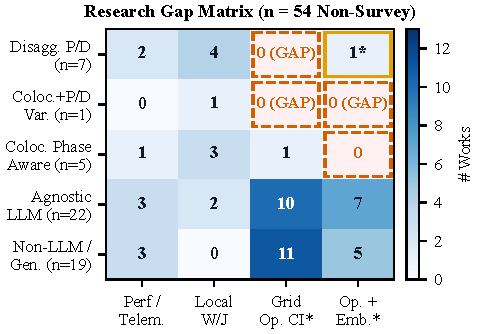
\includegraphics[width=\columnwidth]{figures/fig3_taxonomy_heatmap.pdf}
    \caption{Intersection of phase awareness and carbon/energy signal across $n=38$ non-survey works. *Grid Op. CI includes 10 grid-CI systems plus 2 with battery/water co-signals~\cite{souza2023ecovisor,qi2024casa}; *Op. + Embodied includes 8 operational+embodied works plus CPU aging~\cite{hewage2025aging}.}
    \label{fig:heatmap}
\end{figure}

\begin{figure}[t]
    \centering
    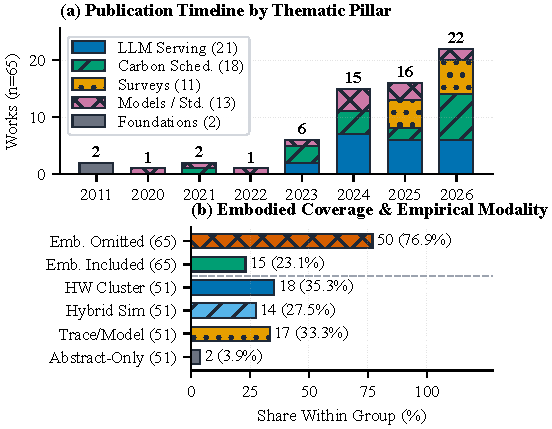
\includegraphics[width=\columnwidth]{figures/fig4_publication_trends.pdf}
    \caption{Corpus bibliometrics from 2011 to 2026 ($n=47$): (a) surge in 2024--2026 output (48.9\% in 2025--2026); (b) 78.7\% embodied omission and empirical evaluation split ($n=35$).}
    \label{fig:trends}
\end{figure}

\begin{table*}[t]
\centering
\caption{Synthesis Comparison Across Empirical Scheduling, LLM Serving, and Lifecycle Carbon Categories (\texttt{L1.B--L1.F})}
\label{tab:matrix}
\scriptsize
\setlength{\tabcolsep}{2.5pt}
\begin{tabular}{@{}p{4.6cm}lllccccp{3.6cm}@{}}
\toprule
\textbf{Category / Representative Works} & \textbf{Class} & \textbf{Scope} & \textbf{Phase} & \textbf{Grid CI} & \textbf{Emb.} & \textbf{KV WAN} & \textbf{Keep-Alive} & \textbf{Primary Knobs / Metrics} \\
\midrule
Wait Awhile~\cite{wiesner2021letswait}, CarbonScaler~\cite{hanafy2023carbonscaler}, EcoVisor~\cite{souza2023ecovisor}, Clover~\cite{li2023clover} & L1.B & Single DC & Non-LLM & \checkmark & $\times$ & $\times$ & $\times$ & Temporal shift, MIG, batteries \\
GreenCourier~\cite{chadha2023greencourier}, Sukprasert~\cite{sukprasert2024limitations}, Caribou~\cite{gsteiger2024caribou}, Calavaro~\cite{calavaro2026offloading}$^\dagger$ & L1.B & Multi-DC & Non-LLM & \checkmark & $\times$ & $\times$ & $\times$ & Geo-routing, HTTP/DAG hops, LP \\
Shahrad~\cite{shahrad2020serverless}, CASA~\cite{qi2024casa}, EcoLife~\cite{jiang2024ecolife}, LowCarb~\cite{roy2026lowcarb}$^\dagger$, LACE-RL~\cite{sun2026lacere}$^\ddagger$ & L1.C & Serverl. & Non-LLM & \checkmark & EcoLife & $\times$ & \checkmark & Dynamic TTL, water+CI, DQN \\
ServerlessLLM~\cite{fu2024serverlessllm}, Festina~\cite{wang2026festina}$^\ddagger$ & L1.C & Serverl. & Agnostic/P/D & $\times$ & $\times$ & $\times$ & \checkmark & NVMe Direct I/O, MPS, DVFS \\
vLLM~\cite{kwon2023vllm}, Sarathi~\cite{agrawal2024sarathi}, Wilkins~\cite{wilkins2024offline}, ThrottLL'eM~\cite{kakolyris2025throttllem} & L1.D & Engine & Agnostic/Col. & $\times$ & $\times$ & $\times$ & $\times$ & PagedAttn, chunking, NVML cap \\
DynamoLLM~\cite{stojkovic2025dynamollm}, TAPAS~\cite{stojkovic2025tapas}, Fernandez et al.~\cite{fernandez2025acl} & L1.D & Cluster & Coloc.\ Phase & Dynamo & $\times$ & $\times$ & $\times$ & Multi-loop DVFS, TP, power cap \\
Splitwise~\cite{patel2024splitwise}, DistServe~\cite{zhong2024distserve}, Mooncake~\cite{qin2025mooncake}, DualScale~\cite{basit2026dualscale}$^\ddagger$, Li~\cite{li2026revisiting}$^\ddagger$ & L1.D & Intra-DC & Disagg.\ P/D & $\times$ & $\times$ & Intra-DC & $\times$ & P/D pools, 50\% cap, MPC, RDMA \\
Gupta~\cite{gupta2021chasing,gupta2022act}$^\dagger$, CarbonExplorer~\cite{acun2023carbonexplorer}, LLMCarbon~\cite{faiz2024llmcarbon}, ISO~\cite{iso2024sci}, Sinha~\cite{sinha2025utilization}$^\dagger$ & L1.E & Lifecycle & Agnostic/Gen. & \checkmark & \checkmark & $\times$ & $\times$ & SCI Eq.~\eqref{eq:sci}, die/HBM capex \\
EcoServe~\cite{li2025ecoserve}$^\ddagger$, Hewage et al.~\cite{hewage2025aging} & L1.E & Cluster & Agnostic & \checkmark & \checkmark & $\times$ & $\times$ & 4R lifetimes (9/3~yr), NBTI aging \\
NIST~\cite{mell2011nist}, CloudSim~\cite{calheiros2011cloudsim}$^\dagger$, Azure Trace~\cite{azure2024trace} & L1.F & Found. & Spec./Trace & $\times$ & $\times$ & $\times$ & $\times$ & Taxonomy, Cloud sim, conv/code logs \\
\midrule
\textbf{This Work (\texttt{P4} Cluster + \texttt{S3} Serverless)} & \text{--} & \textbf{Multi-DC} & \textbf{Disagg.\ P/D} & \checkmark & \checkmark & \checkmark & \checkmark & \textbf{Hybrid A--D, SCI, GapHazard} \\
\bottomrule
\multicolumn{9}{@{}l@{}}{\scriptsize $^\dagger$Abstract-only verified (5 works in corpus). $^\ddagger$Preprint / accepted conference preprint (EcoServe, DualScale, Li et al., LACE-RL, Festina).}
\end{tabular}
\end{table*}
